\documentclass[10pt]{article}
\usepackage[T1]{fontenc}
\usepackage[utf8]{inputenc}

\usepackage{tikz}
\usetikzlibrary{backgrounds,calc}
\usepackage{url}

\begin{document}

\section{Picture-Umgebung in \LaTeX}

\url{http://en.wikibooks.org/wiki/LaTeX/Picture}\\[2cm]

\subsection{Line Segments}

\verb+ \put(x, y){ \line(x1, y1){length} } + 

\begin{figure}[h]
\centering
\setlength{\unitlength}{5cm}
\begin{picture}(1,1)
\put(0,0){\line(0,1){1}}
\end{picture}
\caption{Alle möglichen Steigungen}
\end{figure}

\subsection{Arrows}
\verb+\put(x, y){\vector(x1, y1){length}}+
\begin{figure}
\centering
\setlength{\unitlength}{0.75mm}
\begin{picture}(60,40)
\put(30,20){\vector(1,0){30}}
\end{picture}
\caption{Pfeile}
\end{figure}

\subsection{Circles}
\verb+\put(x, y){\circle{diameter}}+
\begin{figure}[h]
\centering
\setlength{\unitlength}{1mm}
\begin{picture}(60, 40)
\put(20,30){\circle{1}}
\put(35,10){\circle*{5}}
\end{picture}
\caption{Circles}
\end{figure}


\subsection{Mulitput}
\verb+ \multiput(x, y)(dx, dy ){n}{object}+

\begin{figure}[h]
\centering
\setlength{\unitlength}{2mm}
\begin{picture}(30,20)
\linethickness{0.075mm}
\multiput(0,0)(1,0){26}{\line(0,1){20}}
\end{picture}
\caption{Multiput}
\end{figure}

\begin{figure}[h!]
\centering
\setlength{\unitlength}{0.9cm}
\begin{picture}(10,10)(-5,-5)

\put(0,-4.5){\vector(0,1){9}}
\put(-4.5,0){\vector(1,0){9}}
\put(4.8,-0.2){\( x \)}

\put(-3,3){\line(1,0){6}}
\put(3,-3){\line(0,1){6}}
\put(-3,-3){\line(0,1){6}}
\put(-3,-3){\line(1,0){6}}
\put(-4,-4){\line(1,1){8}}

\multiput(-0.1,-4)(0,1){9}{\line(1,0){0.2}}
\multiput(-4,-0.1)(1,0){9}{\line(0,1){0.2}}
\multiput(0.2,0)(0.2,0){14}{\line(0,1){3}}
\end{picture}
\caption{Beispiel für eine direkt mit \LaTeX{} erstellte Grafik\label{fig:picture}}
\end{figure}

\begin{figure}
\centering
\setlength{\unitlength}{1cm}
\begin{picture}(6,6)(-2,-3)

\put(0,-3.2){\vector(0,1){6.4}}
\put(-2.2,0){\vector(1,0){5.4}}
\put(3.4,-0.2){\makebox{$x$}}
\put(2,2){\oval(4,2)[lt]}

\put(0,3){\line(1,0){3}}
\put(3,0){\line(0,1){3}}
\put(-2,-2){\vector(1,1){5.2}}

\multiput(-0.1,-3)(0,1){7}{\line(1,0){0.2}}
\multiput(-2,-0.1)(1,0){6}{\line(0,1){0.2}}
\multiput(0.2,0)(0.2,0){14}{\line(0,1){3}}
\end{picture}
\end{figure}

\section{Kleines TikZ-Beispiel}

\begin{figure}
\centering
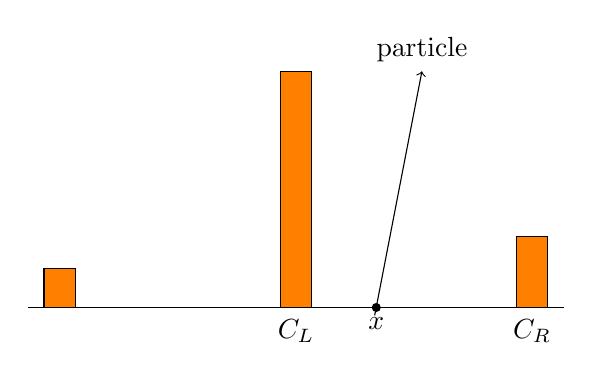
\begin{tikzpicture}
\draw (-3.4,0) -- (3.4,0);
\draw[fill = orange] (-3.2,0) rectangle (-2.8,0.5);
\draw[fill = orange] (-0.2,0) rectangle (0.2,3);
\node at (0,-0.3) {$C_L$};
\draw[fill = orange] (2.8,0) rectangle (3.2,0.9);
\node at (3,-0.3) {$C_R$};
\draw[->] (1,-0.1) -- (1.6,3) node[right,above]{particle};
\draw[fill] (1.02,0) circle [radius=0.05] node[below]{$x$};
\end{tikzpicture}
\caption[Schematic of charge sharing]{Schematic of a charge deposited between two strips $C_{L,R}$. On the far left some charge is registered due to capactive coupling}
\label{fig:schematic}
\end{figure}

\listoffigures
\end{document}